 \thispagestyle{gocconone}
\pagestyle{gocco}
\everymath{\color{gocco}}
\graphicspath{{../gocco/pic/}}
\blfootnote{$^1${\color[named]{gocco}Đại kiện tướng quốc tế.}}
\begingroup
\AddToShipoutPicture*{\put(0,616){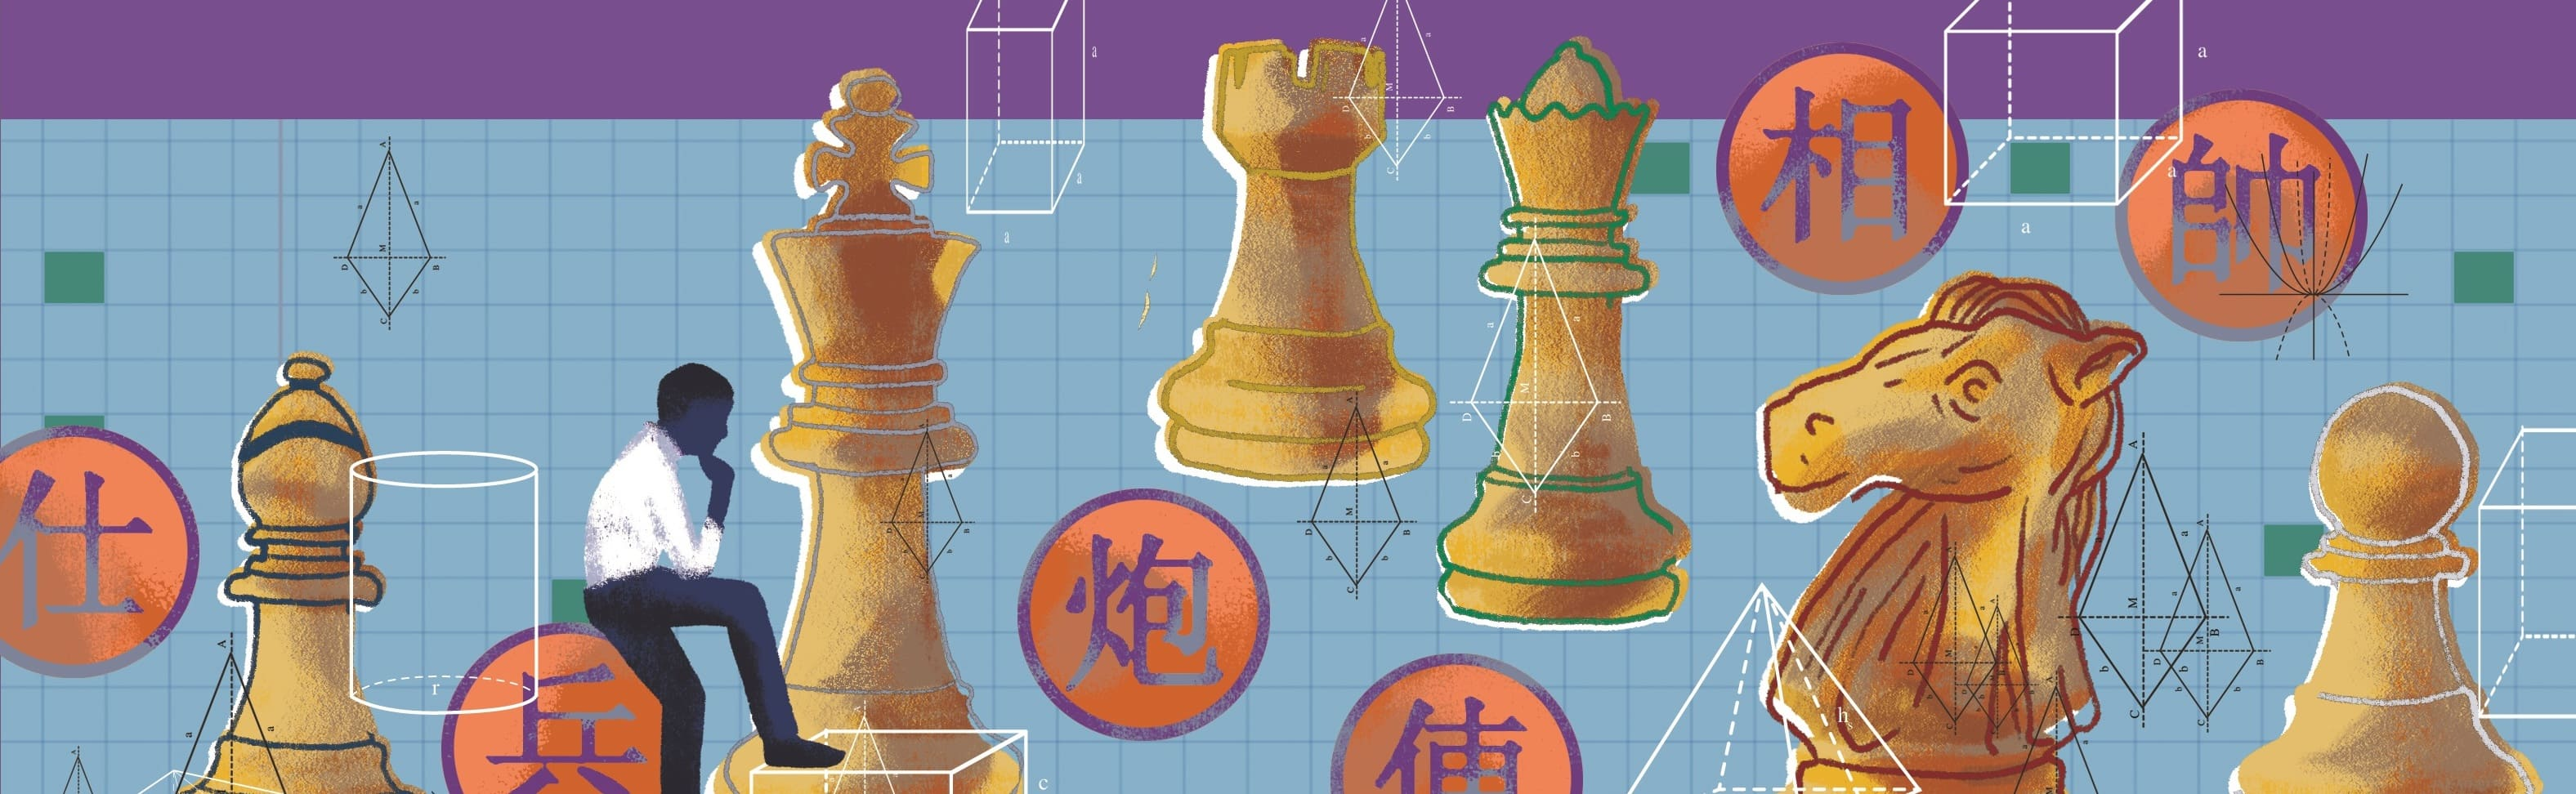
\includegraphics[width=19.3cm]{../bannergocco}}}
\AddToShipoutPicture*{\put(175,553){
\includegraphics[scale=1]{../tieude2.pdf}}} 
\centering
\endgroup

\vspace*{155pt}
\begin{multicols}{2}
	Lý thuyết cờ tàn cơ bản đều cho rằng Hậu sẽ dễ dàng dành chiến thắng khi chống lại xe.
	\vskip 0.1cm
	Trong bài học hôm nay, chúng tôi xin trình bày những kiến thức cờ cơ bản trong từng tình huống cụ thể.
	\vskip 0.1cm
	\textit{$1.$ Trường hợp Hậu chống lại Xe không có tốt.}
	\vskip 0.1cm 
	Hầu hết các trường hợp bên có Hậu (bên mạnh) giành chiến thắng rất dễ dàng. Kế hoạch chiến thắng của bên mạnh là dùng Hậu và vua của mình tìm mọi cách buộc bên có xe phải di chuyển xe khỏi vua, khi đó bên có Hậu sẽ dễ dàng thực hiện nước chiếu bắt~xe.
	\vskip 0.1cm
	\textbf{\color{gocco}Ví dụ $\pmb{1}$: A. Philidor $\pmb{1777}$.}
	\begin{center}
		\newgame
		\fenboard{1k6/1r6/2K5/Q7/8/8/8/8 b Q - 0 1}
		\scalebox{0.85}\showboard
		\vskip 0.1cm
		\textit{\small\color{gocco}Hình $1$.}
		\vspace*{-5pt}
	\end{center}
	\textbf{\color{gocco}Đen đi trước.}
	\vskip 0.1cm
	$\pmb{1}$\textbf{\color{gocco}...Xb}$\pmb{3}$ [Mọi phương án khác của đen đều không thể tránh mất xe như:]
	\vskip 0.1cm
	[$1$...Xb$2$ $2$.He$5+$; $1$...Xb$1$ $2$.Hd$8+$ Va$7$ $3$.Hd$4+$ Va$8$ $4$.Hh$8+$ Va$7$ (\textit{$4$...Xb$8$ $5$.Ha$1\#$}) $5$.Hh$7+$; $1$...Xg$7$ $2$.He$5+$; $1$...Xa$7$ $2$.Hd$8\#$; $1$...Xf$7$ $2$.He$5+$ Va$7$ $3$.He$3+$ Vb$8$ $4$.He$8+$; $1$...Xh$7$ $2$.He$5+$ Va$7$ $3$.Ha$1+$ Vb$8$ $4$.Hb$1+$
	$1$..Vc$8$ $2$. Ha$6$]
	\vskip 0.1cm
	$\pmb{2}$\textbf{\color{gocco}.Hd$\pmb{8+}$ Va$\pmb{7}$ $\pmb{3}$.Hd$\pmb{4+}$ Vb$\pmb{8}$ $\pmb{4}$.Hf$\pmb{4+}$ Va}$\pmb{8}$ [$4$...Va$7$ $5$.Ha$4+$]
	\vskip 0.1cm
	$\pmb{5}$\textbf{\color{gocco}.Ha}$\pmb{4+}$
	\vskip 0.1cm
	Trong khi đó, nếu được đi trước bên Trắng cũng thắng dễ dàng bằng
	\vskip 0.1cm
	$1$. He$5$ Va$8$ $2$. Ha$1$ Vb$8$ $3$. Ha$5$ đen bị bí nước đi.
	\vskip 0.1cm
	$1-0$
	\vskip 0.1cm
	\textbf{\color{gocco}Ví dụ $\pmb{2}$: Y Averbakh $\pmb{1972}$}
	\begin{center}
		\newgame
		\fenboard{5Q2/3k4/8/4r3/2K5/8/8/8 b Q - 0 1}
		\scalebox{0.85}\showboard
		\vskip 0.1cm
		\textit{\small\color{gocco}Hình $2$.}
	\end{center}
	Kế hoạch giành chiến thắng cơ bản của trắng là dùng Hậu và vua ép vua đối phương vào góc bàn cờ, khi đó Xe buộc phải rời khỏi vị trí mà vua đen đang bảo vê. Trắng sẽ thực hiện đòn chiếu bắt xe.
	\vskip 0.1cm
	$\pmb{1}$\textbf{\color{gocco}.Hf$\pmb{7+}$ Vd}$\pmb{6}$ [$1$...Xe$7$ $2$.Hf$5+$ Vd$6$ $3$.Hd$5+$ Vc$7$ $4$.Vc$5$ Xd$7$ $5$.He$5$+ Vb$7$ $6$.Vb$5$ Xc$7$ $7$.Hd$5+$ Va$7$ $8$.Va$5$]
	\vskip 0.1cm
	$\pmb{2}$\textbf{\color{gocco}.Hf}$\pmb{6+}$ [Nước cờ tiêu chuẩn để bắt xe đối phương rời khỏi hàng $5$]
	\vskip 0.1cm
	$\pmb{2}$\textbf{\color{gocco}...Xe$\pmb{6}$ $\pmb{3}$.Hf$\pmb{4+}$ Vc$\pmb{6}$ $\pmb{4}$.Hd}$\pmb{4}$ [Trắng đe dọa Hd$5$ chiếu bắt xe]
	\vskip 0.1cm
	$\pmb{4}$\textbf{\color{gocco}...Xd$\pmb{6}$ $\pmb{5}$.He$\pmb{4+}$ Vb$\pmb{6}$ $\pmb{6}$.Vb$\pmb{4}$ Xc}$\pmb{6}$ [$6$...Xd$7$ $7$.He$6+$ Vc$7$ $8$.Vc$5$ Trắng từ từ dồn vua đen vào góc]
	\vskip 0.1cm
	$\pmb{7}$\textbf{\color{gocco}.Hd$\pmb{4+}$ Va$\pmb{6}$ $\pmb{8}$.Hd$\pmb{8}$ Vb}$\pmb{7}$ [$8$...Xb$6+$ $9$.Vc$5$ Xb$5+$ $10$.Vc$6$; $8$...Xc$1$ $9$.Hd$3+$ Vb$7$ $10.$Vb$5$]
	\vskip 0.1cm
	$\pmb{9}$\textbf{\color{gocco}.Vb}$\pmb{5}$ (Hình $3$)
	\begin{center}
		\newgame
		\fenboard{3Q4/1k6/2r5/1K6/8/8/8/8 b Q - 0 1}
		\scalebox{0.85}\showboard
		\vskip 0.1cm
		\textit{\small\color{gocco}Hình $3$.}
	\end{center}
	$\pmb{9}$\textbf{\color{gocco}...Xc}$\pmb{7.}$ \textbf{\color{gocco}Nước đi duy nhất} Đen không có nước nào tốt hơn, nếu chạy xe khỏi vị trí vua bảo vệ xe bị Hậu trắng chiếu bắt xe. Nếu $9$..Xc$3$ $10$, Hd$5+$ Vc$8$ $11$. Va$6!$ Xc$1$ $12$. Hf$5$ và nước sau chiếu bắt xe.
	\vskip 0.1cm
	$\pmb{10}$\textbf{\color{gocco}.Hd$\pmb{5+}$ Va$\pmb{7}$ $\pmb{11}$.Va$\pmb{5!}$ Xb$\pmb{7}$ $\pmb{12}$.Hd$\pmb{4+}$ Vb$\pmb{8}$ $\pmb{13}$.Va$\pmb{6}$ Xc$\pmb{7}$ $\pmb{14}$.Hd$\pmb{8+}$ Xc$\pmb{8}$ $\pmb{15}$.Hb$\pmb{6+}$ Va$\pmb{8}$ $\pmb{16}$.Hb}$\pmb{7\#}$
	\vskip 0.1cm
	$2$. \textit{Hậu chống lại Xe và tốt}
	\vskip 0.1cm
	Khi có thêm tốt, cơ hội gỡ hòa của bên có xe tăng lên đáng kể phụ thuộc vào vị trí của tốt.
	\vskip 0.1cm
	Nếu như Xe và tốt phối hợp với Vua có thể tự bảo vệ lẫn nhau, bên có Hậu sẽ không thể giành chiến thắng được.Ví dụ dưới đây cho thấy rõ điều đó
	\vskip 0.1cm
	\textbf{\color{gocco}Ví dụ $\pmb{3}$: NN}
	\begin{center}
		\newgame
		\fenboard{1k6/1p6/2r5/1K6/4Q3/8/8/8 b Q - 0 1}
		\scalebox{0.85}\showboard
		\vskip 0.1cm
		\textit{\small\color{gocco}Hình $4$.}
		\vspace*{-5pt}
	\end{center}
	Trắng đi trước, nếu đánh giá tương quan lực lượng cho thấy bên có Hậu mạnh hơn. Tuy nhiên ưu thế của họ không đủ để chiến thắng vì bên đen có thể phòng thù bằng cách xây lô cốt.]
	\vskip 0.1cm
	$\pmb{1}$\textbf{\color{gocco}.He$\pmb{8+}$ Va$\pmb{7}$ $\pmb{2}$.Hd$\pmb{7}$ Xa$\pmb{6}$ $\pmb{3}$.Vc$\pmb{5}$ Xc$\pmb{6+}$ $\pmb{4}$.Vd$\pmb{5}$ Xa$\pmb{6}$ $\pmb{5}$.Hc$\pmb{7}$ Xc$\pmb{6}$ $\pmb{6}$.Ha$\pmb{5+}$ Vb}$\pmb{8}$ (Hình $5$)
	\begin{center}
		\newgame
		\fenboard{1k6/1p6/2r5/Q2K4/8/8/8/8 b Q - 0 1}
		\scalebox{0.85}\showboard
		\vskip 0.1cm
		\textit{\small\color{gocco}Hình $5$.}
		\vspace*{-5pt}
	\end{center}
	Với việc bên đen có $2$ ``điểm tựa"  cho xe là c$6$ và a$6$ do tốt bảo vệ, trắng không có cách nào đưa vua tiếp cận tốt b$7$ cũng như bắt xe đối phương phải di chuyển sang ô cờ mà không được quân đen nào bảo vệ.]
	\vskip 0.1cm
	$\pmb{7}$\textbf{\color{gocco}.Hd$\pmb{8+}$ Va$\pmb{7}$ $\pmb{8}$.Hd$\pmb{7}$ Xa}$\pmb{6}$ [$8$...Va$8$ Phương án này cũng hòa]
	\vskip 0.1cm
	\textbf{\color{gocco}Ví dụ $\pmb{5}$: A.	Philidor $\pmb{1777}$.}
	\begin{center}
		\newgame
		\fenboard{1Q6/3pk3/4r3/5K2/8/8/8/8 b Q - 0 1}
		\scalebox{0.8}\showboard
		\vskip 0.1cm
		\textit{\small\color{gocco}Hình $6$.}
		\vspace*{-5pt}
	\end{center}
	\textbf{\color{gocco}Trắng đi trước và hòa cờ}
	\vskip 0.1cm
	Trong tình huống này bên yếu có $2$ điểm tựa dành cho xe là ô c$6$ và e$6$, từ đó Bên đen dễ dàng gỡ hòa nhờ việc ngăn chặn vua Trắng tiếp cận tốt d$7$.
	\vskip 0.1cm
	$\pmb{1}$.Vg$\pmb{5}$ Xc$\pmb{6}$ $\pmb{2}$.Vf$\pmb{5}$ Xe$\pmb{6}$ $\pmb{3}$.Hb$\pmb{4+}$ Ve$\pmb{8}$ $\pmb{4}$.Hh$\pmb{4}$ Xc$\pmb{6}$ $\pmb{5}$.Hh$\pmb{8+}$ Ve$\pmb{7}$ $\pmb{6}$.Hg$\pmb{7+}$ Ve$\pmb{8}$
	\vskip 0.1cm
	$1/2 - 1/2$
	\vskip 0.1cm
	\textbf{\color{gocco}Ví dụ $\pmb{6}$: V. Khenkin $\pmb{1981}$}
	\begin{center}
		\newgame
		\fenboard{3Q4/3p4/3kr3/5K2/8/8/8/8 b Q - 0 1}
		\scalebox{0.8}\showboard
		\vskip 0.1cm
		\textit{\small\color{gocco}Hình $7$.}
		\vspace*{-5pt}
	\end{center}
	\textbf{\color{gocco}Trắng đi trước thắng}
	\vskip 0.1cm
	Tình huống chúng ta xem ở dưới đây cho thấy vua đen nằm ở ô d$6$ và vô tình đã càn đường xe của mình di chuyển sang ``điểm tựa c$6$"
	\vskip 0.1cm
	Trắng tận dụng được vị trí sai lầm của vua đen và giành chiến thắng.
	\vskip 0.1cm
	$\pmb{1}$\textbf{\color{gocco}.Vg$\pmb{5}$ Xe}$\pmb{2}$ [Xe đen bắt buộc phải di chuyển khỏi ô e$6$]
	\vskip 0.1cm
	[$1$...Vc$6$ $2$.Hb$8!$]
	\vskip 0.1cm
	$\pmb{2}$\textbf{\color{gocco}.Vf$\pmb{4}$ Xf}$\pmb{2+}$ [$2$...Xe$6$ $3$.Vf$5$]
	\vskip 0.1cm
	$\pmb{3}$\textbf{\color{gocco}.Ve$\pmb{3}$ Xc$\pmb{2}$ $\pmb{4}$.Vd$\pmb{3}$ Xc}$\pmb{6}$ [$4$...Xa$2$ $5$.Hb$6+$ Ve$7$ $6$.Hb$4+$ Vd$8$ $7$.Hh$4+$ Ve$8$ $8$.Hf$6!$ Trắng thắng vì đen không thể nào tìm được ô cờ an toàn tránh nước chiếu bắt xe $8$...Xa$5$ $9$.Vc$4$ Xa$2$ $10$.Vb$5$ Xe$2$ $11$.Hh$8+$ Ve$7$ $12$.Hh$4+$ Vd$6$ (\textit{$12$...Ve$8$ $13$.Hh$5+$; $13$...Ve$6$ $14$.Hg$4+$}) $13$.Hb$4+$ Ve$5$ (\textit{$13$...Vd$5$ $14$.Hc$4+$; $12$...Ve$6$ $13$.Hc$4+$; $12$...Vc$7$ $13$.Hc$4+$}) $20$.Qe$7+$]
	\vskip 0.1cm
	$\pmb{5}$\textbf{\color{gocco}.Vd}$\pmb{4!}$ [Hình $8$]
	\begin{center}
		\newgame
		\fenboard{3Q4/3p4/2rk4/8/3K4/8/8/8 b Q - 0 1}
		\scalebox{0.8}\showboard
		\vskip 0.1cm
		\textit{\small\color{gocco}Hình $8$.}
	\end{center}
	$\pmb{5}$\textbf{\color{gocco}...Xc}$\pmb{2}$ [$5$...Xc$1$ $6$.Hf$6+$ Vc$7$ $7$.Hf$4+$]
	\vskip 0.1cm
	$\pmb{6}$\textbf{\color{gocco}.Ha$\pmb{5}$ Xc$\pmb{7}$ $\pmb{7}$.Hd$\pmb{5+}$ Ve$\pmb{7}$ $\pmb{8}$.He$\pmb{5+}$ Vd$\pmb{8}$ $\pmb{9}$.Ha$\pmb{5!}$ Vc}$\pmb{8}$ [$9$...d$6$ $10$.Vd$5$ Vd$7$ $11$.Hb$5+$ Ve$7$ Đen buộc phải cố gắng giữ tốt d$6$. $12$.He$2++–$ Vd$7$ $13$.He$6+$ Vd$8$ Trắng cần phải hết sức cẩn thận vì đen có thể gỡ hòa do hết nước đi $14$.Hg$8+!$ (\textit{Sai lầm nếu $14$.Vxd$6$?? Xc$6+$ $15$.Xxc$6$}. Hòa cờ do hết nước đi; \textit{$14$.Hxd$6+$?? Xd}$7$) $14$...Vd$7$ $15$.Hg$7+$ Vd$8$ $16$.Hf$8+$ Vd$7$ $17$.Hxd$6+$]
	\vskip 0.1cm
	$\pmb{10}$\textbf{\color{gocco}.Ha}$8\#$
	\vskip 0.1cm
	\textbf{\color{gocco}Bài tập: Trắng đi trước thắng}
	\begin{center}
		\newgame
		\fenboard{8/8/k7/p2Q4/1r6/2K5/8/8 b Q - 0 1}
		\scalebox{0.8}\showboard
		\vskip 0.1cm
		\textit{\small\color{gocco}Hình $9$.}
	\end{center}
\end{multicols}




